\section{8.6. More on Sampling}


% SLIDE CHUYỂN PHẦN 8.6
\begin{frame}{Nội dung trình bày}
	\tableofcontents[currentsection]
\end{frame}

% SLIDE 8
\begin{frame}{8.6. Lấy mẫu (Sampling)}
	\textbf{Sự cân bằng (Trade-off):}
	\begin{itemize}
		\item Các phương pháp lấy mẫu luôn phải \textbf{cân bằng} giữa hai yếu tố quan trọng: \textbf{chất lượng (quality)} và \textbf{sự đa dạng (diversity)}.
	\end{itemize}
	
	\vspace{0.5cm}
	
	\textbf{Phân tích:}
	\begin{itemize}
		\item \textbf{Thiên về xác suất cao:} Tạo ra văn bản \textbf{chính xác, mạch lạc} và bám sát thực tế, nhưng thường \textbf{nhàm chán và lặp lại}.
		\item \textbf{Thiên về xác suất trung bình:} Tăng tính \textbf{sáng tạo và đa dạng}, nhưng tiềm ẩn rủi ro \textbf{thiếu liên kết} hoặc chất lượng thấp.
	\end{itemize}
	
\end{frame}

% SLIDE 9
% SLIDE 1: Phần Text
\begin{frame}{8.6.1. Phương pháp Lấy mẫu Top-k}
	\textbf{Khái niệm cốt lõi:}
	\begin{itemize}
		\item Là sự \textbf{tổng quát hóa} của \textbf{Greedy Decoding}.
	\end{itemize}
	
	\vspace{0.4cm}
	\textbf{Thuật toán thực thi:}
	\begin{enumerate}
		\item \textbf{Chọn trước} tham số $k$.
		\item \textbf{Tính Likelihood} cho mọi từ.
		\item Sắp xếp và \textbf{chỉ giữ lại $k$ từ} có xác suất cao nhất.
		\item \textbf{Chuẩn hóa lại (Renormalize)} và \textbf{lấy mẫu ngẫu nhiên} từ $k$ từ này.
	\end{enumerate}
\end{frame}

% SLIDE 2: Phần Hình ảnh
\begin{frame}{8.6.1. Phương pháp Lấy mẫu Top-k}
	\centering
	% Hình placeholder tự thêm
	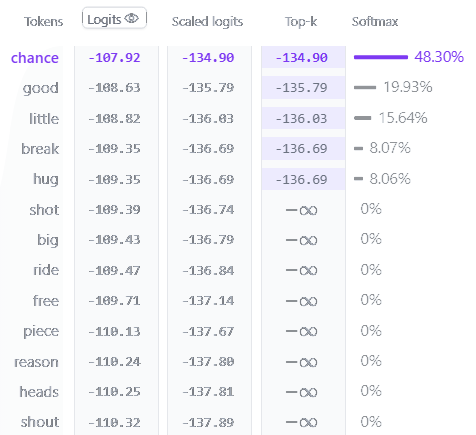
\includegraphics[width=0.9\textwidth, height=0.75\textheight, keepaspectratio]{img/minh_hoa_cat_duoi_top_k_sampling_modified.png}
	\\ \vspace{0.2cm} \scriptsize{Minh họa cắt xén phân phối bằng Top-k, với $k = 5$}
\end{frame}

% SLIDE 3: Phần Text
\begin{frame}{8.6.2. Nucleus Sampling (Top-p) - Vấn đề của Top-k}
	\textbf{Hạn chế của Top-k:}
	\begin{itemize}
		\item Tham số $k$ là \textbf{cố định (fixed)}, trong khi hình dạng phân phối xác suất lại \textbf{thay đổi theo ngữ cảnh}.
	\end{itemize}
	
	\vspace{0.4cm}
	\textbf{Giải pháp Top-p:}
	\begin{itemize}
		\item Thay vì đếm số lượng từ, hệ thống giữ lại \textbf{top $p$ phần trăm} của \textbf{khối lượng xác suất (probability mass)}.
	\end{itemize}
\end{frame}

% SLIDE 4: Phần Hình ảnh
\begin{frame}{8.6.2. Nucleus Sampling (Top-p) - Vấn đề của Top-k}
	\centering
	% Hình placeholder tự thêm
	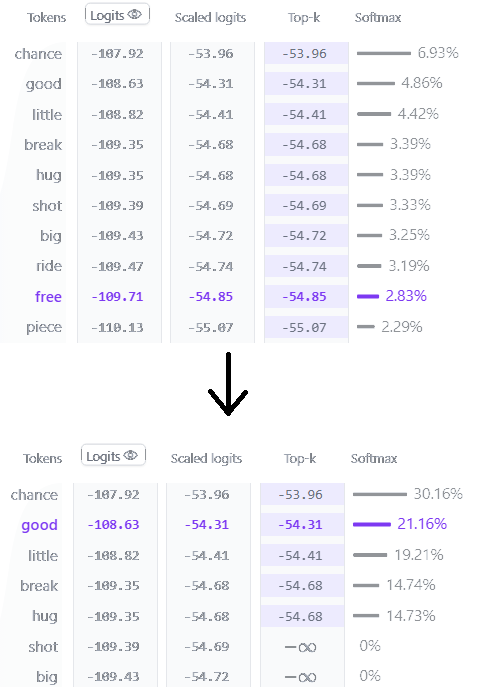
\includegraphics[width=0.9\textwidth, height=0.75\textheight, keepaspectratio]{img/hinh_dang_phan_phoi_thay_doi_theo_ngu_canh_modified.png}
	\\ \vspace{0.2cm} \scriptsize{Sự thay đổi phân phối xác suất khi $k=50 \xrightarrow{} k=5$}
\end{frame}

% SLIDE 5: Phần Text
\begin{frame}{8.6.2. Nucleus Sampling (Top-p)}
	\textbf{Mục tiêu:}
	\begin{itemize}
		\item \textbf{Cắt bỏ phần đuôi phân phối} (các từ rất ít có khả năng xảy ra).
		\item Giúp tập chứa ứng viên \textbf{linh hoạt tùy độ tự tin} của mô hình.
	\end{itemize}
	
	\vspace{0.4cm}
	\textbf{Phương trình tối ưu:}
	\begin{block}{Xác định tập từ vựng $V^{(p)}$}
		Lựa chọn \textbf{tập hợp nhỏ nhất} thỏa mãn:
		\begin{equation*}
			\sum_{w \in V^{(p)}} P(w | w_{<t}) \ge p
			\tag{8.48}
			\label{eq:top_p}
		\end{equation*}
	\end{block}
\end{frame}

% SLIDE 6: Phần Hình ảnh
\begin{frame}{8.6.2. Nucleus Sampling (Top-p)}
	\centering
	% Hình placeholder tự thêm
	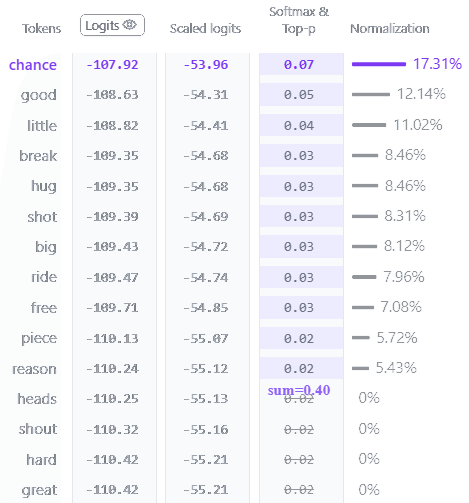
\includegraphics[width=0.9\textwidth, height=0.75\textheight, keepaspectratio]{img/minh_hoa_tich_luy_xac_suat_top_p_modified.png}
	\\ \vspace{0.2cm} \scriptsize{Minh họa bao phủ khối lượng xác suất Top-p}
\end{frame}

